\usecaseristoratore{Accetta prenotazione}
\label{usecase:Accetta prenotazione}

\begin{figure}[h]
	\centering
	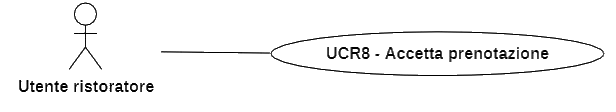
\includegraphics[width=0.8\textwidth]{./uml/UCR8.png} 
	\caption{Accetta prenotazione}
	\label{fig:UCR8}
  \end{figure}

\begin{itemize}
	\item \textbf{Attore principale:} Utente ristoratore.

	\item \textbf{Precondizioni:}
	      \begin{itemize}
		      \item L'Utente ristoratore visualizza la prenotazione in dettaglio (vedi \autoref{usecase:Visualizza dettaglio lista prenotazioni}).

		      \item La prenotazione è nello stato "In attesa".
	      \end{itemize}

	\item \textbf{Postcondizione:} L'Utente ristoratore accetta la prenotazione.


	\item \textbf{Scenario principale:}
	      \begin{enumerate}
		      \item L'Utente ristoratore seleziona l'opzione di accettazione della prenotazione;

		      \item Il Sistema aggiorna lo stato della prenotazione.
	      \end{enumerate}
\end{itemize}
